\documentclass{article}
\usepackage{graphicx}

\graphicspath{{images/}}
\begin{document}

\title{A0--MinMax Algorithm Analysis}
\author{Michael Fulton}
\date{February 3, 2015}

\maketitle

\section{Recursive Analysis}

	The function which relates cost functions to number of inputs for my recursive algorithm is as follows:

\[
	C(N)=
	\begin{cases}
		2C(\frac{N}{2})+2 \mbox{ if} N < 2 \\
		1 \mbox{ if}   N = 2 \\
		0 \mbox{ if} \leq 1 
	\end{cases}
\]


\[f(n) = \begin{cases} n/2 \mbox{if } n \equiv 0 \\ 
(3n +1)/2  \mbox{if } n \equiv 1. \end{cases}\]

	
\section{Iterative Analysis}

\newpage
\section{Plots}
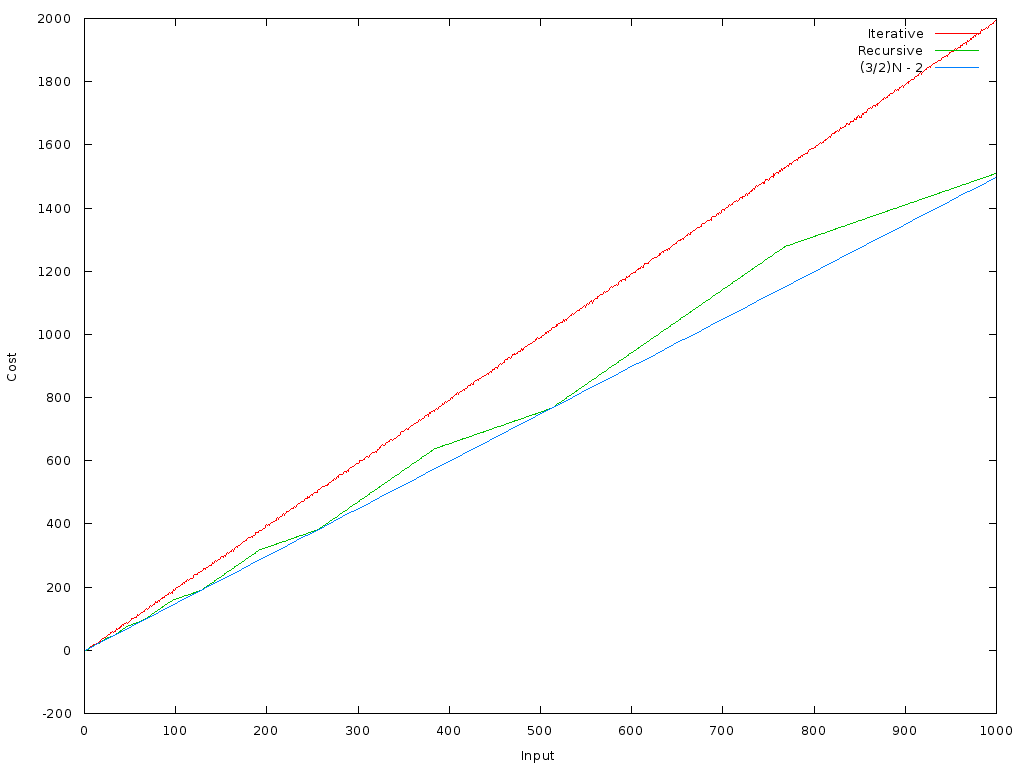
\includegraphics[scale =0.6]{plot.png}
\centering

\end{document}
